\raggedbottom
\subsection{Auditory Processing Disorder}
\gls{apd} is a neurological condition that affects a child's ability to accurately process and interpret auditory information. Individuals with \gls{apd} may have difficulty distinguishing sounds, recognizing speech patterns, understanding spoken language, and filtering out background noise. To develop interventions tailored to the needs of children with an auditory processing disorder, it is important to understand their unique user profile. This includes identifying their specific goals, psychographics, problems, characteristics and needs related to auditory processing and communication. Figure \ref{fig:APDUserProfile} represents the \gls{apd} user profile.

\begin{figure}[H]
    \centering
    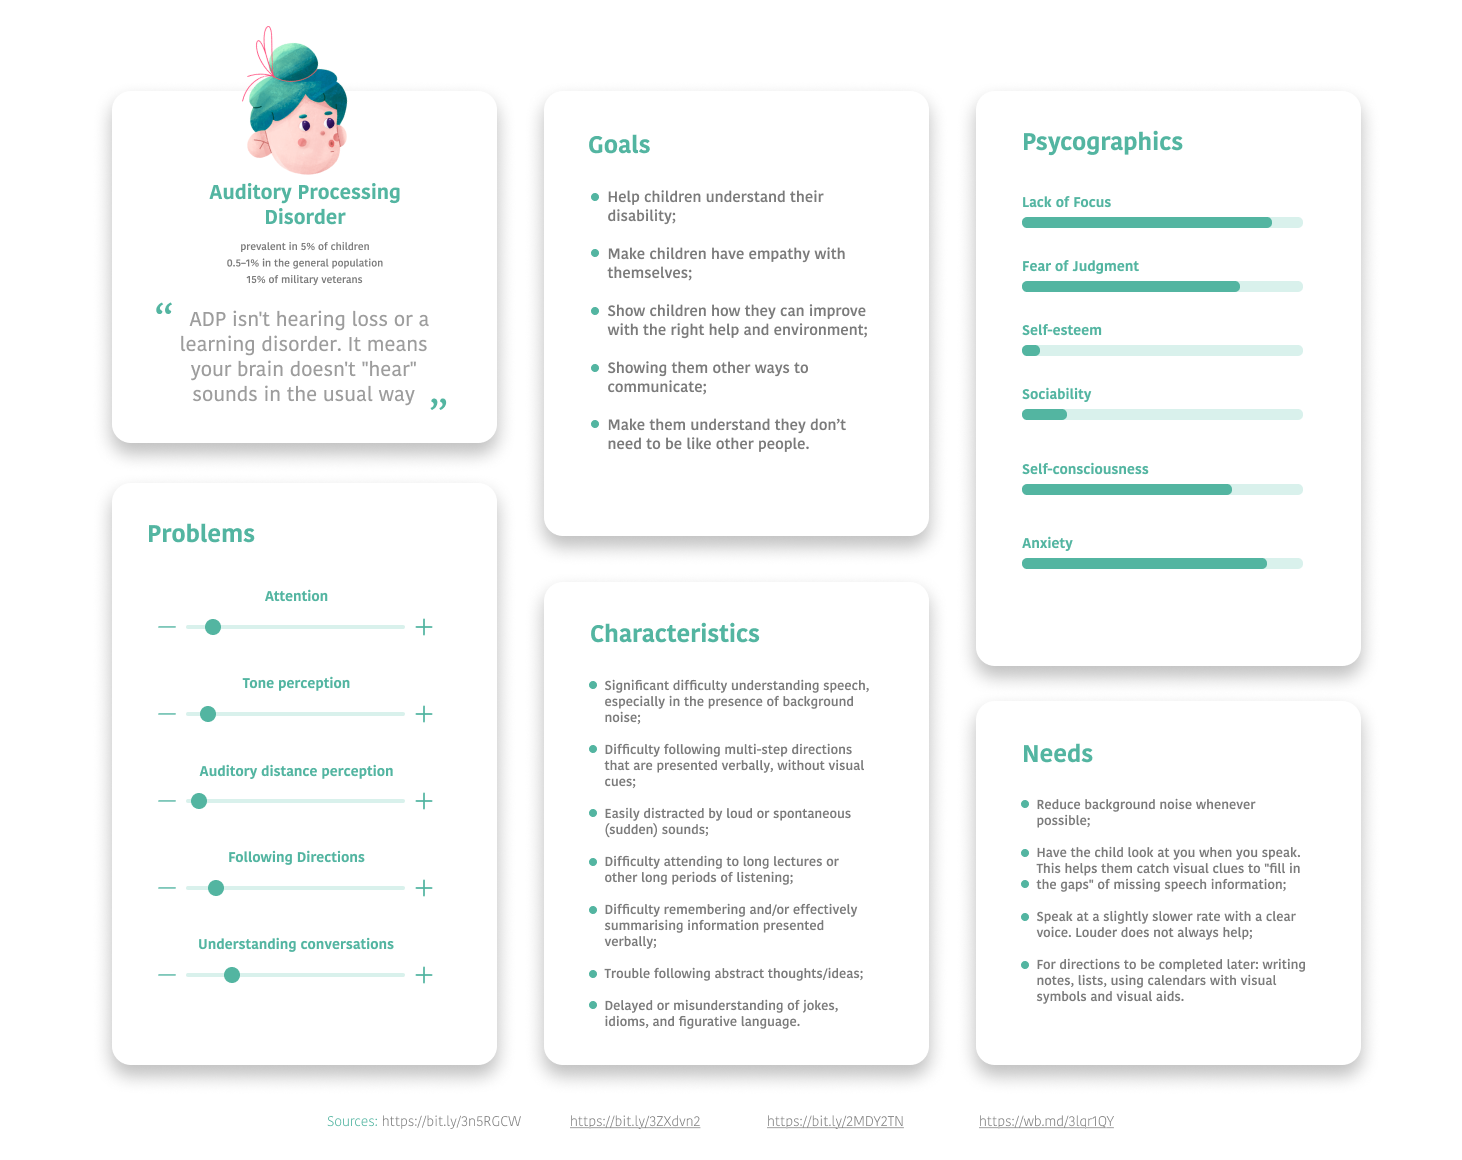
\includegraphics[width=1\linewidth]{Chapters/figma/Auditory Processing Disorder.png}
    \caption{Auditory Processing Disorder User Profile}
    \label{fig:APDUserProfile}
\end{figure}

\paragraph{Goals}
\begin{itemize}
    \item \textbf{Help children understand their disability}: The mini-games aim to provide children with a comprehensive understanding of \gls{apd}, including its impact on their auditory processing skills and the specific challenges they may face in communication and comprehension.
    \item \textbf{Foster empathy and self-acceptance}: By creating an environment of empathy and self-acceptance, the mini-games aim to help children develop a positive self-image, embrace their unique auditory processing abilities, and build resilience in the face of auditory challenges.
    \item \textbf{Show children how they can improve}: The mini-games should demonstrate to children that with the right help, strategies, and supportive environment, they can improve their auditory processing skills and effectively navigate through various listening situations.
    \item \textbf{Provide alternative communication methods}: The mini-games aim to explore and provide children with alternative ways to communicate and comprehend information beyond traditional auditory channels.
    \item \textbf{Promote self-acceptance}: The mini-games should emphasize that children with \gls{apd} do not need to compare themselves against others and that their unique auditory processing abilities are valuable in their own right.
\end{itemize}

\paragraph{Psychographics}
\begin{itemize}
    \item \textbf{Low self-esteem}: Struggles with self-worth and confidence, often influenced by difficulties in understanding and responding appropriately to spoken language \cite{KidsHealth}.
    \item \textbf{Low sociability}: Tendency to withdraw from social interactions due to challenges in understanding and participating in conversations \cite{KidsHealth}.
    \item \textbf{High lack of focus}: Difficulty maintaining attention and concentration in auditory tasks due to the challenges in processing auditory information accurately \cite{Nationwide}.
    \item \textbf{High fear of judgment}: Anxiety and fear of being misunderstood or judged by others due to difficulties in comprehending verbal instructions or conversations \cite{KidsHealth}.
    \item \textbf{High self-consciousness}: Heightened awareness of their auditory difficulties and how they may be perceived by others \cite{KidsHealth}.
    \item \textbf{High anxiety}: Experiencing elevated levels of anxiety, particularly in situations involving complex auditory input or noisy environments \cite{KidsHealth}.
\end{itemize}

\paragraph{Problems}
\begin{itemize}
    \item \textbf{Attention}: Difficulties in sustaining attention and focus on auditory tasks, particularly in the presence of background noise or competing stimuli \cite{HearingHealth}.
    \item \textbf{Tone perception}: Challenges in accurately perceiving and interpreting subtle variations in tone and intonation in spoken language, affecting the ability to understand emotions, sarcasm, or subtle nuances in communication \cite{Nationwide}.
    \item \textbf{Auditory distance perception}: Difficulties in accurately perceiving the distance or location from which sounds originate, which can lead to challenges in localizing sounds or distinguishing relevant auditory cues \cite{KidsHealth}.
    \item \textbf{Following directions}: Difficulty comprehending and remembering multi-step directions or instructions that are presented verbally, without visual cues \cite{Nationwide}.
    \item \textbf{Understanding conversations}: Struggles in processing and comprehending conversations, especially in situations with multiple speakers, fast-paced speech, or complex language structures \cite{Nationwide}.
\end{itemize}

\paragraph{Characteristics}
\begin{itemize}
    \item \textbf{Significant difficulty understanding speech, especially in the presence of background noise}: Struggling to extract relevant information from auditory stimuli, leading to challenges in understanding speech in noisy environments \cite{Nationwide}.
    \item \textbf{Difficulty following multi-step directions without visual cues}: Finding it challenging to retain and follow verbal instructions that involve multiple steps or complex sequencing \cite{WebMD}.
    \item \textbf{Easily distracted by loud or spontaneous sounds}: Exhibiting heightened sensitivity to environmental sounds and being easily overwhelmed by unexpected or sudden auditory stimuli \cite{Nationwide}.
    \item \textbf{Difficulty attending to long lectures or extended periods of listening}: Struggling to sustain attention and focus during lengthy auditory tasks, such as lectures or extended conversations \cite{Nationwide}.
    \item \textbf{Difficulty remembering and summarizing information presented verbally}: Challenges in retaining and accurately summarizing information presented in spoken form, impacting learning and information processing \cite{Nationwide}.
    \item \textbf{Trouble following abstract thoughts and ideas}: Finding it challenging to grasp abstract concepts or complex ideas conveyed through spoken language \cite{Nationwide}.
    \item \textbf{Delayed or misunderstanding of jokes, idioms, and figurative language}: Difficulties in comprehending and interpreting humor, idiomatic expressions, metaphors, and figurative language, which rely heavily on auditory processing skills \cite{Nationwide}.
\end{itemize}

\paragraph{Needs}
\begin{itemize}
    \item \textbf{Reduce background noise whenever possible}: Creating an auditory environment with minimal distractions and background noise to optimize the child's ability to focus on and process auditory information \cite{Nationwide}.
    \item \textbf{Encourage visual cues}: Promoting the use of visual cues, such as maintaining eye contact, gestures, facial expressions, and visual aids, to supplement auditory input and enhance comprehension \cite{Nationwide}.
    \item \textbf{Modify speech delivery}: Speaking at a slightly slower rate with a clear and distinct voice, ensuring that instructions and information are presented in a manner that facilitates comprehension for children with \gls{apd}. Louder speech may not necessarily help and can potentially increase sensory overload \cite{KidsHealth}.
    \item \textbf{Provide visual supports}: Utilizing visual supports, such as written notes, lists, calendars with visual symbols, and visual aids, to reinforce verbal information and assist with memory recall and organization \cite{KidsHealth}.
    \item \textbf{Offer alternative communication methods}: Incorporating alternative modes of communication, such as visual or written responses, within the mini-games to accommodate the needs and preferences of children with \gls{apd} \cite{KidsHealth}.
    \item \textbf{Individualize learning experiences}: Designing mini-games such that they can adapt to the unique learning profile of each child with \gls{apd}, providing personalized challenges and support to foster growth and skill development \cite{KidsHealth}.
\end{itemize}

